\documentclass[conference]{IEEEtran}
\IEEEoverridecommandlockouts

% ==========================================
% PACKAGES
% ==========================================
\usepackage{cite}
\usepackage{amsmath,amssymb,amsfonts}
\usepackage{algorithmic}
\usepackage{graphicx}
\usepackage{textcomp}
\usepackage{xcolor}
\usepackage{booktabs}
\usepackage{multirow}
\usepackage{url}
\usepackage{float}
\usepackage{listings}

% --- TIKZ & PLOTS ---
\usepackage{tikz}
\usetikzlibrary{shapes.geometric, arrows, positioning, fit, calc, backgrounds, shadows}

% --- FORMATTING CONFIGURATION ---
\def\BibTeX{{\rm B\kern-.05em{\sc i\kern-.025em b}\kern-.08em
    T\kern-.1667em\lower.7ex\hbox{E}\kern-.125emX}}

% Ensure strict formatting
\setlength{\textfloatsep}{10pt plus 1.0pt minus 2.0pt}
\renewcommand{\baselinestretch}{1.0} 

\begin{document}

% ==========================================
% TITLE
% ==========================================
\title{Architectural Irreversibility: Enforcing Privacy, Governance, and Trust in Intelligent Campus Systems}

% ==========================================
% AUTHOR
% ==========================================
\author{\IEEEauthorblockN{Dr. S. Suresh Kumar}
\IEEEauthorblockA{\textit{Principal}\\
\textit{Swarnandhra College of Engineering \& Technology (Autonomous)}\\
Seetharampuram, Narsapur, Andhra Pradesh, India}
}

\maketitle

% ==========================================
% ABSTRACT
% ==========================================
\begin{abstract}
Intelligent campus infrastructures now rely increasingly on sensor networks and analytics platforms to support safety, coordination, and operational decision-making. These deployments frequently attempt to reconcile the analytical value of observational data with expanding institutional obligations to preserve individual privacy. While these administrative mechanisms establish an important security baseline, they typically operate within architectures that still retain the technical capacity to collect, persist, and reconstruct high-fidelity biometric information.

This work develops an architectural design principle termed Architectural Irreversibility, in which strict privacy constraints are embedded directly into the computational data pipeline. Rather than relying solely on administrative restraint or retrospective compliance audits, the proposed framework constrains the feasibility of reconstructing sensitive information by forcing data through destructive abstraction boundaries. Because purely technical privacy guarantees rarely generate social trust when they remain invisible, interface-level abstractions are used to communicate these limits directly to affected stakeholders. 

Within this framework, durable public trust emerges from infrastructures that structurally eliminate the ability to observe or retain sensitive information instead of relying solely on administrative restraint.
\end{abstract}

\begin{IEEEkeywords}
Architectural Irreversibility, Capability Elimination, Governance-Embedded Inference, Destructive Abstraction, Monotonic Sensitivity Reduction, Socio-Technical Trust.
\end{IEEEkeywords}

% ==========================================
% I. INTRODUCTION
% ==========================================
\section{Introduction}

The dominant thesis of this paper is that \textbf{privacy is strongest when sensitive observational capability is structurally eliminated rather than administratively governed}. Intelligent campus infrastructures increasingly integrate sensing technologies, edge analytics, and automated decision systems into everyday institutional operations. Despite growing regulatory attention, public reception of pervasive sensing remains ambivalent. This persistent socio-technical tension suggests that conventional policy-driven safeguards fail to address the deeper concern: latent surveillance capability.

\subsection{The Persistence of Reversible Surveillance Architectures}
Most contemporary privacy-preserving AI systems encrypt sensitive data but still retain it. They rely on administrative restraint after collection, preserve reconstructable biometrics in encrypted storage, and maintain latent future surveillance capability behind access-control boundaries. In these architectures, governance occurs only after the dangerous capability already exists. Retrospective protection remains structurally fragile: if highly sensitive biometric data persists in any reconstructable form, the probability of repurposing, leakage, or exploitation increases over time. Architectural elimination differs fundamentally from administrative restriction.

This paper introduces Architectural Irreversibility as a foundational design principle in which strict privacy constraints are embedded directly into the computational data pipeline. Rather than regulating how sensitive data is used after capture, this paradigm structurally constrains whether the system can possess such data at all. Within the ScholarMaster architecture, this subsystem defines irreversible abstraction, capability elimination, governance interposition, and visible boundedness only. It does not validate runtime crash behavior (Paper 18), derive formal adversary theorems (Paper 19), construct distributed compliance logic (Paper 21), synthesize deployment architecture (Paper 20), or perform longitudinal trust analytics (Paper 16).

% ==========================================
% II. PROBLEM REFRAMING
% ==========================================
\section{Problem Reframing: Why Privacy-by-Policy Fails}

To understand why institutional monitoring systems frequently encounter resistance, it is necessary to examine the structural limitations of policy-driven privacy protection.

\subsection{The False Promise of Post-Hoc Privacy}
Many intelligent campus deployments attempt to demonstrate privacy compliance through familiar enterprise security mechanisms. These typically include AES-256 encryption at rest, strict Role-Based Access Control (RBAC), immutable audit logging, and alignment with comprehensive regulatory frameworks like the General Data Protection Regulation (GDPR). Administrators often cite these mechanisms as comprehensive safeguards against misuse. Yet empirical sociological evidence across education, healthcare, and smart-city deployments shows persistent distrust and active resistance even in systems that pass rigorous technical compliance audits \cite{b5}.

The fundamental limitation of this approach is entirely structural: these protections only trigger after sensitive information has been captured, retained, or processed in a reversible form. Encryption secures data that already exists on a storage drive. Access controls merely govern who may interact with data that has already been aggregated. Audit logs simply create a forensic record of how existing data was handled by administrators. None of these administrative mechanisms alter the underlying architectural reality that the system currently possesses detailed, high-fidelity representations of living individuals. 

From a systems engineering perspective, this introduces a dangerous asymmetry because capability always precedes governance. Once an edge node or central server possesses the technical capability to observe, store, and infer sensitive attributes, administrative policies must continually fight a rearguard action to ensure that this capability is never exercised improperly. Experience across large-scale technical infrastructures suggests that such guarantees are highly brittle \cite{b4}. Human error, subtle software misconfigurations, adversarial state-actors, or future institutional repurposing can easily expand the system's use well beyond its originally stated intent. Written policies may regulate human behavior under ideal conditions, yet they do little to remove the underlying technological capability that enables misuse.

\subsection{Data as a High-Liability Asset}
Within large-scale data infrastructures, raw sensory information frequently behaves less like a strategic asset and more like a persistent institutional liability. Within the specific context of biometric and behavioral analytics in educational spaces, however, raw data may be more appropriately modeled as a high-liability or hazardous informational asset \cite{b9}. 

When an educational institution chooses to store detailed video streams or raw acoustic recordings of its student body, it assumes an immense, long-term responsibility for protecting that information. Centralized data lakes immediately become a lucrative target for external cyberattacks, a highly sensitive vector for insider threat abuses, and a massive financial and operational burden during legal discovery processes. If the raw data persists, the institution must allocate continuous capital attempting to secure it against a constantly evolving threat landscape. 

Constraint-embedded design circumvents this liability entirely by refusing to generate the high-liability asset in the first place. If an edge computing node processes sensory input into irreversible, sparse abstractions and immediately discards the raw photographic captures, a total physical or network compromise of that node yields only coarse semantic signals. Attackers retrieve meaningless coordinates and timestamps rather than reconstructable facial biometrics, neutralizing the incentive for the attack.

\subsection{Capability Leakage and Mission Creep}
Centralized data architectures often accumulate latent analytical capability over time. Even if raw biometric data remains unused initially, the mere existence of archived captures enables vast future inference capabilities. Machine learning models can be effortlessly retrained using historical footage to extract entirely new features that were not considered during the initial deployment. Deep behavioral correlations can be discovered years after the data was originally collected. Feature expansions driven by new administrative demands may introduce entirely new analytical objectives that students never explicitly consented to \cite{b12}.

This gradual transformation rarely occurs through a single malicious decision. Instead, it happens through incremental feature creep that appears locally reasonable—perhaps adding a module to track library usage density to optimize HVAC systems, and then later adding another module to monitor exam attention. Collectively, these shifts drastically alter the system's role, turning benign infrastructure into a panoptic tracking grid \cite{b3}. Students and faculty often recognize this risk instinctively. Their resistance to automated monitoring systems is not simply a reactionary fear of unfamiliar technology; it is a highly rational response to architectures that concentrate asymmetric observational power while offering only procedural, paper-based assurances.

\subsection{The Limits of Compliance-Driven Design}
Legal and regulatory frameworks are frequently invoked as definitive proof of system safety. However, regulations inherently govern use, not existence. They specify lawful purposes, mandate maximum retention limits, and outline user rights, but they do not mandate architectural impossibility. 

A monitoring system can be entirely legally compliant while still storing high-resolution biometric video data, provided it secures that data and promises its eventual deletion at the end of the academic term. From a software engineering perspective, this arrangement remains structurally fragile. Compliance also suffers from temporal fragility. Legal frameworks shift rapidly, meaning a system optimized for maximum allowable data retention today could easily fall out of compliance tomorrow following a single judicial ruling. Embedding privacy directly as an immutable architectural property, rather than as a flexible regulatory obligation, drastically reduces the institution's reliance on shifting external governance structures.

% ==========================================
% III. A TAXONOMY OF PRIVACY ARCHITECTURES
% ==========================================
\section{A Taxonomy of Privacy Architectures}

Clarifying the difference between governance mechanisms and structural constraints requires a systematic classification of privacy architectures. Let $C$ represent the surveillance capability of the system, $G$ represent the administrative governance controls, and $A$ represent the underlying physical and software architecture. Three broad, distinct classes emerge from this model.

\textbf{1. Policy-Constrained Systems:}
In this paradigm the system retains the full capability ($C$) to surveil, record, and reconstruct sensitive information. The governance layer ($G$) restricts its use purely through administrative rules, Terms of Service agreements, and legal compliance workflows. The system could easily violate privacy at any time, but it is explicitly instructed not to. The institution relies entirely on the premise that administrators will follow the rules and that the security perimeter will never be breached.

\textbf{2. Cryptographically-Constrained Systems:}
The surveillance capability ($C$) still exists in full fidelity, but $G$, combined with heavy cryptographic encryption, restricts access to the raw data, allowing only authorized key-holders to view it. While the data is considerably safer from outside attackers or casual insider snooping, the institution itself still retains the ultimate capability to decrypt, analyze, and repurpose the data at its own discretion. In practical terms the capability therefore remains latent within the system.

\textbf{3. Architecturally-Constrained Systems:}
In this final paradigm, the capability to perform retrospective surveillance or reconstruct biometric identity simply does not exist within the system state space ($C \notin S$). The architecture ($A$) itself eliminates the mathematical and physical possibility of performing these operations. The system cannot violate privacy, even if ordered to do so by a rogue administrator or compromised by a sophisticated external attacker, because the mathematical capacity to reverse the data has been destroyed at the edge.

This taxonomy highlights the profound difference between merely limiting access to a dangerous capability and eliminating that capability entirely from the design space.

% ==========================================
% IV. ARCHITECTURAL IRREVERSIBILITY
% ==========================================
\section{Architectural Irreversibility}

\subsection{From Reversible Pipelines to Irreversible Systems}
Architectural Irreversibility proposes a fundamental shift in how intelligent systems process sensitive environmental data. Most conventional AI systems are constructed as highly reversible processing pipelines. Raw inputs are ingested, transformed, stored in intermediate databases, and iteratively reprocessed across multiple stages of a network. Even when intermediate representations are generated for specific downstream tasks, the original source data frequently persists in various system caches or backup mechanisms. Such reversibility heavily facilitates software debugging and allows engineers to deploy new feature updates retrospectively. However, it fundamentally conflicts with strict privacy constraints.

Architectural Irreversibility instead proposes a markedly different paradigm centered on destructive transformation. Once a data transformation occurs at the edge node, reconstructing the original sensory input becomes computationally infeasible within the established system boundary.

% --- FIGURE 1: IRREVERSIBILITY PIPELINE ---
\begin{figure}[htbp]
\centering
\resizebox{\columnwidth}{!}{
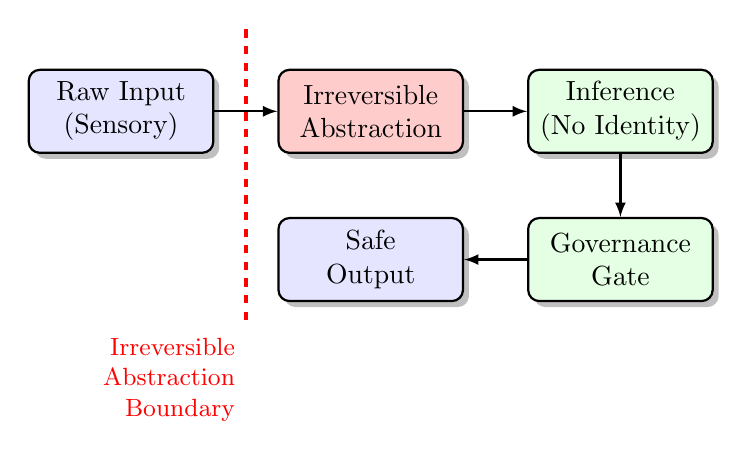
\begin{tikzpicture}[node distance=1.5cm, auto, >=latex, thick]
    % Styles
    \tikzstyle{block} = [rectangle, draw, fill=blue!10, text width=6em, text centered, rounded corners, minimum height=3em, drop shadow]
    \tikzstyle{destruct} = [rectangle, draw, fill=red!20, text width=6em, text centered, rounded corners, minimum height=3em, drop shadow]
    \tikzstyle{safe} = [rectangle, draw, fill=green!10, text width=6em, text centered, rounded corners, minimum height=3em, drop shadow]
    \tikzstyle{line} = [draw, -latex, thick]

    % Nodes
    \node [block] (input) {Raw Input\\(Sensory)};
    \node [destruct, right=0.8cm of input] (destroy) {Irreversible\\Abstraction};
    \node [safe, right=0.8cm of destroy] (infer) {Inference\\(No Identity)};
    \node [safe, below=0.8cm of infer] (govern) {Governance\\Gate};
    \node [block, left=0.8cm of govern] (output) {Safe\\Output};

    % Edges
    \draw [line] (input) -- (destroy);
    \draw [line] (destroy) -- (infer);
    \draw [line] (infer) -- (govern);
    \draw [line] (govern) -- (output);

    % Barrier
    \draw [red, dashed, very thick] ($(input.north east)+(0.4,0.5)$) -- ($(input.south east)+(0.4,-2.2)$) node [below left, text=red, font=\small, align=right] {Irreversible\\Abstraction\\Boundary};
\end{tikzpicture}
}
\caption{The Irreversible Pipeline. Raw data exists exclusively in volatile memory buffers that are never committed to persistent storage. The data is destructively transformed at the abstraction boundary, mathematically preventing reconstruction before higher-order inference occurs.}
\label{fig:pipeline}
\end{figure}

\subsection{The Capability Elimination Principle}
The proposed architecture relies on a central engineering principle termed Capability Elimination---the deliberate removal of unnecessary observational capacity. We distinguish three capability states:
\begin{itemize}
    \item $C_{raw}$: Raw observational capability exists (high-fidelity biometric data is present and accessible).
    \item $C_{abstract}$: Data has been transformed but auxiliary information may still permit partial reconstruction.
    \item $C_{nonreconstructable}$: The transformation is irreversible and all auxiliary side-channel information has been destroyed.
\end{itemize}
The architectural goal is to enforce the irreversible state transition $C_{raw} \rightarrow C_{abstract} \rightarrow C_{nonreconstructable}$ at the edge, before any persistent storage or network transmission occurs. Consider a mathematical transformation applied to a video frame: $f: X \rightarrow Y$. If $f$ is non-invertible, and the original raw state $X$ is actively destroyed, then reconstruction requires external auxiliary information that no longer exists anywhere in the system.

Achieving the $C_{nonreconstructable}$ state requires the coordinated enforcement of several strict engineering conditions: highly non-invertible transformation functions, the complete elimination of raw persistence mechanisms, the absence of key-based recovery, and the strict removal of reversible dense embeddings. Irreversibility depends not only on the algorithmic transformation but also on rigorous system configuration assumptions---secure boot mechanisms and hardened firmware to prevent undocumented side-channel persistence.

\subsection{Relationship to Privacy-Enhancing Technologies}
It is vital to contrast this architectural approach with modern Privacy-Enhancing Technologies (PETs). Frameworks such as Differential Privacy, Federated Learning, and Secure Hardware Enclaves provide incredibly strong protections for existing datasets. They do not, however, eliminate the underlying architectural possibility of raw data collection. They excel at securing data that is already allowed to exist within the boundary. Architectural Irreversibility differs fundamentally: rather than securing data, it prevents the existence of sensitive representations in the first place, ensuring there is no honeypot left to encrypt or federate.

\subsection{The Illusion of De-Identification}
Traditional privacy approaches routinely rely on basic anonymization or pseudonymization. Privacy researchers have conclusively demonstrated, however, that anonymized datasets can almost always be aggressively re-identified through the injection of external, auxiliary information \cite{b20}. Pseudonymized identifiers remain inherently reversible to anyone within the institution who possesses access to the mapping key \cite{b2}. Encrypted data, while safe from outside actors, preserves full biometric fidelity for authorized users inside the institution. All three of these standard techniques preserve the underlying capability to reconstruct sensitive information. Architectural elimination removes that capability entirely from the environment.

\subsection{Dimensionality Reduction as a Mechanism of Privacy}

Within the proposed architecture, privacy arises organically through aggressive, highly entropic dimensionality reduction. High-resolution environmental captures—for example, 4K video frames containing detailed facial structures, unique clothing brands, and identifying physical traits—are mathematically crushed into incredibly sparse semantic vectors before they can be saved.

One practical instantiation of this involves skeletal pose extraction. Instead of storing images of individuals within the lecture hall, the system records only the specific angles of their joints and their relative spatial coordinates. This transformation deliberately discards identifying visual detail while cleanly preserving the behavioral signals required for institutional analytical tasks.

% ==========================================
% V. MANDATORY GOVERNANCE
% ==========================================
\section{Mandatory Governance}

\subsection{Governance as Computational Interposition}
Effective AI governance requires more than policy documentation. In many institutional environments, governance frameworks exist outside the software system itself---in policy documents or compliance checklists. This architecture embeds governance directly into the execution pipeline as compiled code. Governance in this architecture is \textbf{computationally interposed}, not administratively advisory: inference engines cannot directly actuate institutional action. Governance layers constrain execution pathways, and authority separation is embedded into software boundaries. Policy enforcement is implemented in code boundaries that regulate which outputs are permitted to leave the edge node.

\subsection{Epistemic Humility}
Machine learning models produce statistical, probabilistic predictions rather than ground-truth facts. Allowing an AI model to trigger administrative actions directly---for instance, autonomously marking a student as ``disengaged'' based on a posture classification---risks treating uncertain statistical inference as authoritative institutional judgment \cite{b13}. 

The architecture enforces Epistemic Humility \cite{b21} by strictly separating \textit{judgment} (the model's statistical inference) from \textit{authority} (the policy-driven approval to act). The inference engine may judge that a behavior is occurring, but it lacks the authority to broadcast that conclusion. Only a dedicated Governance layer---armed with context-aware institutional policy---possesses the authority to release conclusions beyond the system boundary.

\subsection{Constraint-First Systems Engineering}
Traditional AI systems pursue optimization: maximizing predictive performance at all costs. Architectural Irreversibility adopts a constraint-first systems engineering philosophy. The system is intentionally limited rather than maximally intelligent. The overall utility is deliberately bounded to preserve Nissenbaum's contextual integrity \cite{b4}. When operational uncertainty arises---if the policy verification server becomes unreachable, or if an audit database goes offline---the system defaults to a rigid fail-closed state. Inference results are suppressed and outputs are blocked. This architecture enforces bounded observability, irreversible reduction, fail-closed operation, and constrained inference authority.

% ==========================================
% VI. VISIBLE PRIVACY AND TRUST
% ==========================================
\section{Visible Privacy and Trust}

\subsection{Transparency vs Legibility}
Even mathematically robust privacy guarantees may fail to produce public trust when they remain invisible to system participants. In the design of socio-technical systems, transparency and legibility are often—sometimes dangerously—confused. Publishing source code in a public repository may technically reveal how the system behaves. However, it provides absolutely no psychological reassurance to a non-technical student entering a monitored classroom. Students encountering monitoring infrastructure rarely have the time or expertise to examine source repositories. Their perception of safety depends entirely on the visible, localized behavior of the system as they experience it \cite{b14}.

\subsection{The Semiotics of Abstraction}

To bridge this gap, the architecture heavily restricts user-facing interfaces to purely abstract representations. Instead of providing administrative dashboards that display live RGB video feeds to security personnel, the interfaces are strictly limited to displaying skeletal wireframes, geometric nodes, or de-identified spatial markers mapped onto a blank grid \cite{b19}. 

This visual language communicates an incredibly important, immediate constraint: identity information is physically inaccessible to the human operators viewing the screen. The visual abstraction functions simultaneously as a hard technical privacy mechanism and a potent sociological trust signal. It allows non-technical users to independently verify the system's operational limits through direct observation, rather than forcing them to rely on blind faith in unseen administrative privacy policies.

% ==========================================
% VII. THE ARCHITECTURE OF STEWARDSHIP
% ==========================================
\section{The Architecture of Stewardship}

The principles established above---irreversible transformation, mandatory governance, and visible privacy---are realized through a layered reduction pipeline that systematically eliminates identity dimensions as data ascends through the system. The detailed structural specification, including formal stratum definitions, layer-to-layer execution contracts, and deployment topology mappings, is developed in companion work on reference architecture design (Paper 20). This paper establishes the doctrinal foundations that motivate and constrain that structural specification.

\subsection{Monotonic Sensitivity Reduction as Governing Invariant}
At the conceptual level, the pipeline enforces a strict monotonic reduction in data sensitivity. This property serves as the governing architectural invariant of the entire system. Environmental signals begin as high-entropy, high-fidelity sensory captures at the physical substrate. Each successive conceptual boundary irreversibly strips additional dimensions of identity, behavioral detail, or temporal specificity. Critically, no downstream layer may re-enrich destroyed semantics---abstraction boundaries represent irreversible entropy reduction. By the time information reaches institutional decision-makers, it has been reduced to anonymous, aggregate semantic signals that cannot be traced back to any individual.

The key doctrinal constraints governing this pipeline are:

\begin{itemize}
    \item \textbf{Monotonic Sensitivity Reduction:} Information sensitivity must decrease at every boundary transition. No layer may re-enrich data with identity dimensions that a prior boundary destroyed. This property must hold consistently across pipeline discussion, governance reasoning, and systems framing.
    \item \textbf{Unidirectional Flow:} Data flows exclusively upward through the pipeline. No feedback loop may carry post-boundary abstracted data back to pre-boundary layers where it could be correlated with raw captures.
    \item \textbf{Mandatory Governance Interposition:} No abstracted output may reach external sinks without passing through an explicit, computationally interposed governance evaluation.
    \item \textbf{Fail-Closed Default:} Any boundary failure causes the pipeline to halt rather than degrade into a permissive state.
\end{itemize}

% ==========================================
% VIII. NON-NEGOTIABLE ARCHITECTURAL CONSTRAINTS
% ==========================================
\section{Non-Negotiable Architectural Constraints}

Traditional software systems rely on highly malleable legal agreements and generic Terms of Service to regulate institutional behavior. This framework proposes replacing these fragile legal constructs with non-negotiable architectural invariants. These constraints dictate that the system simply cannot perform certain actions, regardless of the user's administrative privilege level or institutional directives. 

\textbf{Boundary Irreversibility} guarantees that raw sensory data can never cross abstraction boundaries into persistent storage. \textbf{Governance Liveness} mandates that no output can be generated or transmitted without actively passing through dynamic policy approval. \textbf{Algorithmic Forgetting} enforces the continuous, rolling expiration of contextual state, flatly prohibiting the construction of long-term psychological profiles of participants \cite{b16}. Finally, the \textbf{Principle of Least Privilege in Memory} denies persistent storage access to the perception layers entirely. Philosophically, these uncompromising boundaries represent the intentionally designed limits of the machine's agency.

% ==========================================
% IX. ETHICAL POSITIONING
% ==========================================
\section{Ethical Positioning}

\subsection{From Compliance to Constraint}
Architectural Irreversibility represents a transition from compliance-driven governance toward constraint-oriented system design. Compliance frameworks typically describe what systems should not do, leaving open the possibility of human error or malicious override. Architectural constraint defines what systems fundamentally cannot do. By embedding data minimization directly into the system's software and hardware design, we drastically reduce society's reliance on the shifting discretion of institutional administrators \cite{b23}.

\subsection{The Stewardship Model}
Automated Stewardship contrasts deeply with traditional, surveillance-driven data extraction systems. Surveillance architectures inherently prioritize maximum information retention, relying on systemic opacity to maintain a power asymmetry over the observed subjects \cite{b10}. Stewardship architectures, conversely, prioritize harm reduction and system legitimacy through visible, demonstrable constraint \cite{b15}.

\subsection{Practical Trade-offs and Operational Realism}
Irreversible systems introduce real engineering limitations. System debugging becomes substantially more difficult because raw frames are unavailable for forensic review following a model failure. Certain longitudinal analytics tasks requiring historical biometric reconstruction are rendered permanently impossible. These limitations are deliberate trade-offs that prioritize human privacy over analytical convenience. Operationally, institutions must also contend with deployment maintenance complexity: edge-device hardening requirements, firmware trust assumptions, and the overhead of maintaining governance-interposed pipelines across heterogeneous campus hardware.

\subsection{Limitations}
The architectural enforcement of irreversibility and governance constraint introduces several operational boundaries. Under the defined architectural boundary, the following constraints apply:
\begin{itemize}
    \item \textbf{Diagnostic Opacity:} By destructively transforming raw video inputs at the edge, forensic debugging of model misclassifications becomes nearly impossible, as the ground-truth visual data no longer exists.
    \item \textbf{Longitudinal Rigidity:} Irreversibility fundamentally prevents retrospective feature expansion; institutions cannot retroactively train new machine learning models on historical environmental conditions because the raw data was never retained.
    \item \textbf{Hardware Trust Dependency:} The guarantee of irreversibility relies on the physical security of the edge sensing nodes; compromised firmware could bypass the abstraction boundary before destruction occurs. Side-channel leakage may still exist within the constrained execution model.
    \item \textbf{Side-Channel Vulnerability:} Even when raw biometrics are eliminated, highly granular skeletal vectors or metadata flows may still expose unique behavioral signatures vulnerable to complex linkage attacks. The architecture substantially constrains reconstructability but does not claim absolute protection.
    \item \textbf{Asymmetric Development Costs:} Embedding governance directly into compiled pipeline boundaries significantly increases engineering complexity and maintenance cost compared to traditional, permissive data-lake architectures.
\end{itemize}

% ==========================================
% X. CONCLUSION
% ==========================================
\section{Conclusion}

This paper presented Architectural Irreversibility as a bounded architectural doctrine for structural capability elimination in privacy-sensitive campus infrastructures. By embedding one-way abstraction boundaries directly into the computational pipeline, the architecture reduces latent surveillance capability rather than administratively restricting its exercise. The irreversible state transition $C_{raw} \rightarrow C_{abstract} \rightarrow C_{nonreconstructable}$, governed by monotonic sensitivity reduction, ensures that information sensitivity decreases at every pipeline boundary under the defined architectural assumptions.

Visible abstraction interfaces reduce informational asymmetry by allowing non-technical users to observe the system's operational limits directly. Together these mechanisms demonstrate how privacy can be treated as a foundational property of system architecture rather than a retrospective regulatory obligation.

Within the ScholarMaster architecture, this framework operates exclusively as the architectural governance and irreversible privacy subsystem---defining capability elimination, governance interposition, and visible boundedness without validating runtime crash behavior (Paper 18), deriving formal adversary theorems (Paper 19), constructing distributed compliance logic (Paper 21), synthesizing deployment topology (Paper 20), or performing longitudinal trust analytics (Paper 16).

% ==========================================
% REFERENCES
% ==========================================
\begin{thebibliography}{00}

\bibitem{b1} J. Bentham, \textit{The Panopticon Writings}. Verso, 1995.
\bibitem{b2} D. J. Solove, ``A taxonomy of privacy,'' \textit{Univ. of Pennsylvania Law Review}, vol. 154, no. 3, pp. 477--570, 2006.
\bibitem{b3} S. Zuboff, \textit{The Age of Surveillance Capitalism}. PublicAffairs, 2019.
\bibitem{b4} H. Nissenbaum, \textit{Privacy in Context: Technology, Policy, and the Integrity of Social Life}. Stanford Univ. Press, 2009.
\bibitem{b5} F. Pasquale, \textit{The Black Box Society}. Harvard Univ. Press, 2015.
\bibitem{b6} R. C. Mayer, J. H. Davis, and F. D. Schoorman, ``An integrative model of organizational trust,'' \textit{Acad. of Management Review}, vol. 20, no. 3, pp. 709--734, 1995.
\bibitem{b7} J. D. Lee and K. A. See, ``Trust in automation: Designing for appropriate reliance,'' \textit{Human Factors}, vol. 46, no. 1, pp. 50--80, 2004.
\bibitem{b8} J. Penney, ``Chilling effects: Online surveillance and Wikipedia use,'' \textit{Berkeley Tech. Law Journal}, vol. 31, no. 1, 2016.
\bibitem{b9} B. Schneier, \textit{Data and Goliath: The Hidden Battles to Collect Your Data and Control Your World}. W. W. Norton \& Company, 2015.
\bibitem{b10} S. U. Noble, \textit{Algorithms of Oppression}. NYU Press, 2018.
\bibitem{b11} V. Eubanks, \textit{Automating Inequality}. St. Martin's Press, 2018.
\bibitem{b12} N. Couldry and U. A. Mejias, ``Data colonialism,'' \textit{Television \& New Media}, vol. 20, no. 4, pp. 336--349, 2019.
\bibitem{b13} J. Sweller, ``Cognitive load during problem solving,'' \textit{Cognitive Science}, vol. 12, no. 2, pp. 257--285, 1988.
\bibitem{b14} M. R. Endsley, ``Toward a theory of situation awareness,'' \textit{Human Factors}, vol. 37, no. 1, pp. 32--64, 1995.
\bibitem{b15} L. Floridi, \textit{The Ethics of Information}. Oxford University Press, 2013.
\bibitem{b16} R. R. Hoffman et al., ``Accelerated proficiency and facilitated retention,'' \textit{Cognitive Processing}, vol. 14, no. 2, pp. 147--163, 2013.
\bibitem{b18} R. T. Azuma, ``A survey of augmented reality,'' \textit{Presence}, vol. 6, no. 4, pp. 355--385, 1997.
\bibitem{b19} P. Milgram and F. Kishino, ``A taxonomy of mixed reality displays,'' \textit{IEICE Trans. Inf. Syst.}, vol. E77-D, no. 12, pp. 1321--1329, 1994.
\bibitem{b20} L. Sweeney, ``k-anonymity: A model for protecting privacy,'' \textit{International Journal of Uncertainty, Fuzziness and Knowledge-Based Systems}, vol. 10, no. 5, pp. 557-570, 2002.
\bibitem{b21} S. Jasanoff, ``Technologies of Humility: Citizen Participation in Governing Science,'' \textit{Minerva}, vol. 41, no. 3, pp. 223-244, 2003.
\bibitem{b23} A. Cavoukian, ``Privacy by design: The 7 foundational principles,'' Information and Privacy Commissioner of Ontario, 2009.
\bibitem{b24} M. Hildebrandt, \textit{Smart Technologies and the End(s) of Law}. Edward Elgar, 2015.

\end{thebibliography}

\end{document}
